\section{The beam test of chamber E}\label{app:beam}
\sectionstate{partial}{\texttt{sps\_beam\_test\_26/det4\_sps\_assessment} (stripes), \texttt{rerun/sps\_region/README.md} (working region,
position), \texttt{rerun/paper1\_spsfigs} (gas, known angle, footprint). v2 2026-11-10: the old section 9 (stripes), the SPS gas
figure of the old section 6 and the two results that the old section 3.2 promised and nothing showed.}
\intent{This appendix answers: what was measured in the beam, on which part of chamber~E, and how far it can be
trusted as a cross-check of the bench.}

\subsection{The stripes of chamber E, and the working region}\label{sec:det4}
Chamber~E has a production defect that is visible in every data set: stripes of its area do not amplify
(\crefp{fig:effmap}{e}, \cref{fig:det4}).
\tbw{Board map, periodicity, connector and strip-break tests, HV headroom, stability across runs.}
\askStephan{Do the stripes match anything in chamber~E's production (resistive printing, lamination, a particular step)?
Was it seen in QA? Is this paper the place to show it?}
Because of the stripes, every beam number of this paper is measured in one \emph{working region} of full efficiency,
the box R of \cref{fig:det4} (10\,mm in $x$ by 24\,mm in $y$); five other patches in the live bands serve only to
check that it is representative.
\begin{figure}[tbp]
  \centering
  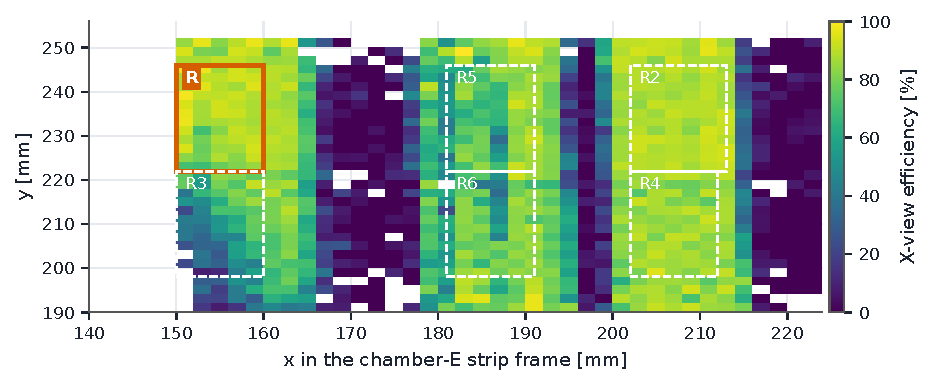
\includegraphics[width=\linewidth]{det4_stripes}
  \caption{Chamber~E in the beam: efficiency map of the X view (2\,mm bins, axes not to scale) from the tracks of the
  reference telescope, in Ar/CF$_4$/iC$_4$H$_{10}$. The non-amplifying stripes are the dark bands. Solid box R: the
  working region in which every beam resolution of this paper is measured (\cref{sec:position}). Dashed boxes R2--R6:
  other patches of similar size in the live bands, used only to check that R is representative.}
  \label{fig:det4}
\end{figure}

\subsection{Angle scale and charge footprint}
Two further beam results are reported in the companion paper~\cite{paperII} and only quoted here. With the chamber
yawed by 25.4\textdegree{} and the drift velocity taken from the duration of the drift column, the fitted angle of the
inclined view is $0.981\pm0.03$ of the known one. At normal incidence, in data taken without zero suppression, a strip
next to the leading strip carries 0.38 (X) and 0.39 (Y) of its amplitude, independently of the drift field from 96 to
243\,V/cm, so the footprint is not diffusion.
\askDylan{The old section 3.2 promised both and no section showed them. They are companion-paper figures
(\texttt{known\_angle}, \texttt{kernel\_forms}); quoted here in two sentences, or drop them.}

\subsection{The gas in the beam}\label{app:beamgas}
The gas analysis of \cref{sec:gas} applied to each group of beam runs gives the water and the oxygen of chamber~E
against time (\cref{fig:attach}). The chamber ran wetter than on the bench, at 1.7 to 2.1\,\% of water, and with 130 to
440\,ppm of oxygen, which is what makes its drift column fall with time (\cref{sec:attachment}).
\begin{figure}[tbp]
  \centering
  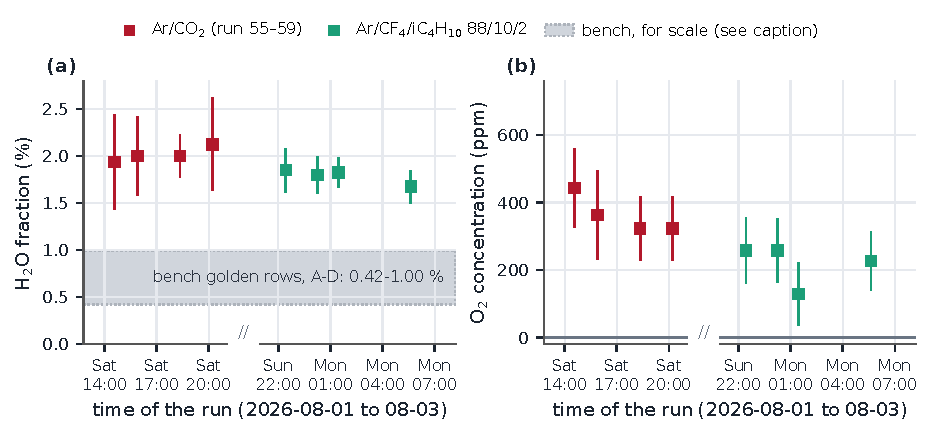
\includegraphics[width=\linewidth]{attachment}
  \caption{Gas of chamber~E in the beam, from the drift columns of tracks at normal incidence with a 27.9\,mm gap,
  against the time of each group of runs (the 22 idle hours between Saturday evening and Sunday night are cut): (a)
  water, (b) oxygen (red: Ar/CO$_2$; green: Ar/CF$_4$/iC$_4$H$_{10}$ 88/10/2). With the geometric gap of chamber~E,
  28.6\,mm, the water is 0.1--0.2\,\% lower. Grey band in (a): the water of the long runs on the bench, 0.42--1.00\,\%
  for the five chambers.}
  \label{fig:attach}
\end{figure}
\askDylan{The label printed inside panel (a) of \cref{fig:attach} still reads ``bench golden rows, A--D''; the band includes
chamber~E (0.42\,\%), so it should read ``bench, chambers A--E''. A one-line change in \texttt{rerun/paper1\_spsfigs/attach\_fig.py};
not made, because that script belongs to the paper1 figure set.}
